\section{Regulador de amplitud de oscilación}
Según el paper REFERENCIA para una celda del orden de los centímetros entre placas es conveniente usar 1V de amplitud. Para bajarlo de $6.84V$ a $1V$ se propuso una configuración inversora que deberá tener una ganancia de $\dfrac{1}{6.84}=0.146 V/V$ por lo tanto se eligió  $R5=100\Omega$ y $R8$ un preset de $1k\Omega$ para tener la posibilidad de calibrar la amplitud.
\section{Multiplexor analógico}

Se ve la necesidad de utilizar el mismo circuito para medir la conductividad de la leche de cada cuarto y de este modo ahorrar componentes. Para ello se plantea utilizar un multiplexor analógico conectado como el que se muestra en la figura \ref{fig:mux}, donde $R_{mi}$ son las resistencias equivalentes de cada cuarto de leche.

\begin{figure}[H]
\centering
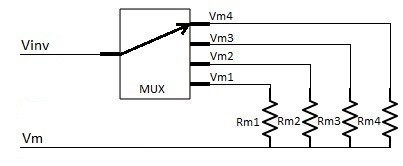
\includegraphics[width=0.6\textwidth]{mux/mux.jpg}
\caption{Diagrama conexionado del multiplexor}
\label{fig:mux}
\end{figure}

Se necesita un multiplexor que tenga por lo menos cuatro salidas y como la señal $V_{inv}$ varía entre $\pm 1V$, se necesita que pueda excursionar entre $\pm 1V$. Por lo que se elige el 74HC4052 que cumple con estos requerimientos.\\

En la figura \ref{fig:mux_pins} se observa el diagrama de pines del multiplexor. $VCC$ y $VEE$ son la alimentación y fijan los limites de excursión. Según la la hoja de datos alimentándolo en $\pm 4.5V$ la resistencia de condución es de $65\Omega$ típico, esta resistencia va a estar en serie con la de la leche por lo tanto le quita sensibilidad a la medida. Razón por la cual se selecciona la celda de $R_{m} $ mayor.\\

Se cuenta con dos patas digitales de control ($S0$ y $S1$) para elegir la salida. Una pata digital que conecta o desconecta la entrada ($E$). Este multiplexor está compuesto por dos multiplexores de cuatro salidas que funcionan en paralelo comandados por las patas digitales mencionadas anteriormente, las entradas son ($1Z$ $2Z$) y las correspondientes salidas son ($1Yi$ $2Yj$), en nuestro caso se necesita solo uno de estos multiplexores.


\begin{figure}[H]
\centering
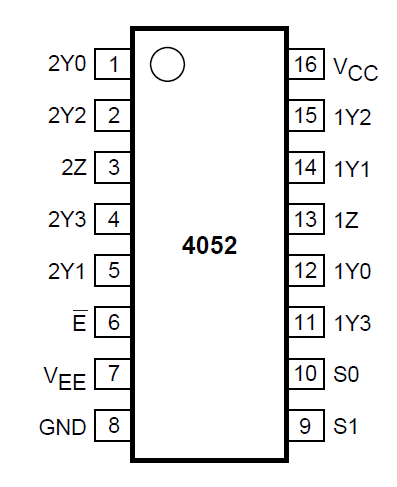
\includegraphics[width=0.4\textwidth]{mux/mux_pins.png}
\caption{Pines del multiplexor}
\label{fig:mux_pins}
\end{figure}


\section{Amplificador de conductividad}
Para poder aprovechar la presicion de la entrada analógica de arduino es deseable que en el máximo esperado de conductividad el voltaje de salida sea el máximo que permite la entrada de arduino (5V).\\

La resistencia equivalente de la celda con leche es:\\
\begin{equation}
R_{m} =\dfrac{l}{\sigma S}
\label{eq:Rm}
\end{equation}
Donde $l$ es la distancia entre las placas, $S$ es la sección de las placas y $\sigma$ es la conductividad de la leche.\\

Dado que se selecciona la celda 2 que tiene dimensiones $l=2cm$, $a=0.5cm$ y $h=1cm$ se tiene $S=0.5cm^{2}$. En REFERENCIA, la conductividad máxima esperada es de $\sigma_{m}=9 mS/cm$ por lo tanto $R_{m}=444\Omega$. La entrada es de $1V$ y se desea tener $5V$ a la salida por lo tanto la transferencia debe tener una ganancia de $5V/V$. En una configuración inversora, el módulo de la transferencia es $\dfrac{R_{10}}{R_{m}}=5$ entonces $R_{10}=2.2k\Omega$.  Pero se utiliza un preset de $5k\Omega$ para poder calibrar la ganancia.